\chapter{O pedaço escolhido}\label{cap:pedaco}

O andar anterior mediu o que não se compra. Este abre o andar do enquadramento, e começa pela coisa
que atravessou a espiral inteira sem ser discutida: \textbf{a série}. Toda pergunta desta obra foi
respondida sobre uma série, e a série tem começo e fim porque alguém escolheu onde eles ficam.

\section{A resposta de um pedaço só}

A medição é a do primeiro capítulo, que é a mais simples que a espiral tem: quantos dias rompem o
corte de \numPedacoJanela{} dias. A promessa é de \numPedacoPromessa{}, e o teste usa
\numPedacoTamanhos{} tamanhos de pedaço, até \numPedacoMaior{} dias.

A mesma conta, feita em pedaços de \numPedacoMenor{} dias ao longo dos \numPedacoDiasA{} dias do
índice --- \numPedacoDiasComuns{} dias em comum com a segunda perna ---, dá de \numPedacoEntregaMenorDoisAnos{} a \numPedacoEntregaMaiorDoisAnos{}: a maior resposta é
\numPedacoEntregaRazaoDoisAnos{} vezes a menor. Nenhuma das duas está errada, e as duas são o mesmo
mercado.

\begin{table}[htbp]
  \centering
  \small
  \begin{tabular}{rrrrrr}
    \hline
    pedaço & número de & menor & maior & dispersão & a conta \\
    (dias) & pedaços & resposta & resposta & medida & independente \\
    \hline
    \numPedacoMenor{} & \numPedacoPedacosDoisAnos & \numPedacoEntregaMenorDoisAnos & \numPedacoEntregaMaiorDoisAnos & \numPedacoEntregaDispersaoDoisAnos & \numPedacoEntregaIndependenteDoisAnos \\
    mil duzentos e sessenta & \numPedacoPedacosCincoAnos & \numPedacoEntregaMenorCincoAnos & \numPedacoEntregaMaiorCincoAnos & \numPedacoEntregaDispersaoCincoAnos & \numPedacoEntregaIndependenteCincoAnos \\
    dois mil quinhentos e vinte & \numPedacoPedacosDezAnos & \numPedacoEntregaMenorDezAnos & \numPedacoEntregaMaiorDezAnos & \numPedacoEntregaDispersaoDezAnos & \numPedacoEntregaIndependenteDezAnos \\
    \hline
  \end{tabular}
  \caption{A entrega do corte medida em pedaços de três tamanhos. A última coluna é o que a conta de
    sempre prevê para a dispersão entre pedaços, que é a conta de quem supõe dias independentes:
    $\sqrt{p(1-p)/n}$.}
  \label{tab:pedacos}
\end{table}

A tabela tem duas leituras. A primeira é a largura: a resposta muda por um fator de mais de dez
entre a menor e a maior da primeira linha. A segunda é a distância entre a coluna medida e a coluna
da conta --- \numPedacoEntregaDispersaoDoisAnos{} contra
\numPedacoEntregaIndependenteDoisAnos{}, mais de três vezes. A conta independente é a que se faria
se cada dia fosse um sorteio novo; os dias do mercado não são, e a diferença é o preço de supor que
fossem. A razão entre a maior e a menor resposta cai de \numPedacoEntregaRazaoDoisAnos{}, nos pedaços
de dois anos, para \numPedacoEntregaRazaoCincoAnos{} e \numPedacoEntregaRazaoDezAnos{} nos maiores ---
que é o que se espera, e a calma tem preço: um pedaço grande o bastante para dar a resposta certa
também esconde o quanto ela mudou.

\begin{figure}[htbp]
  \centering
  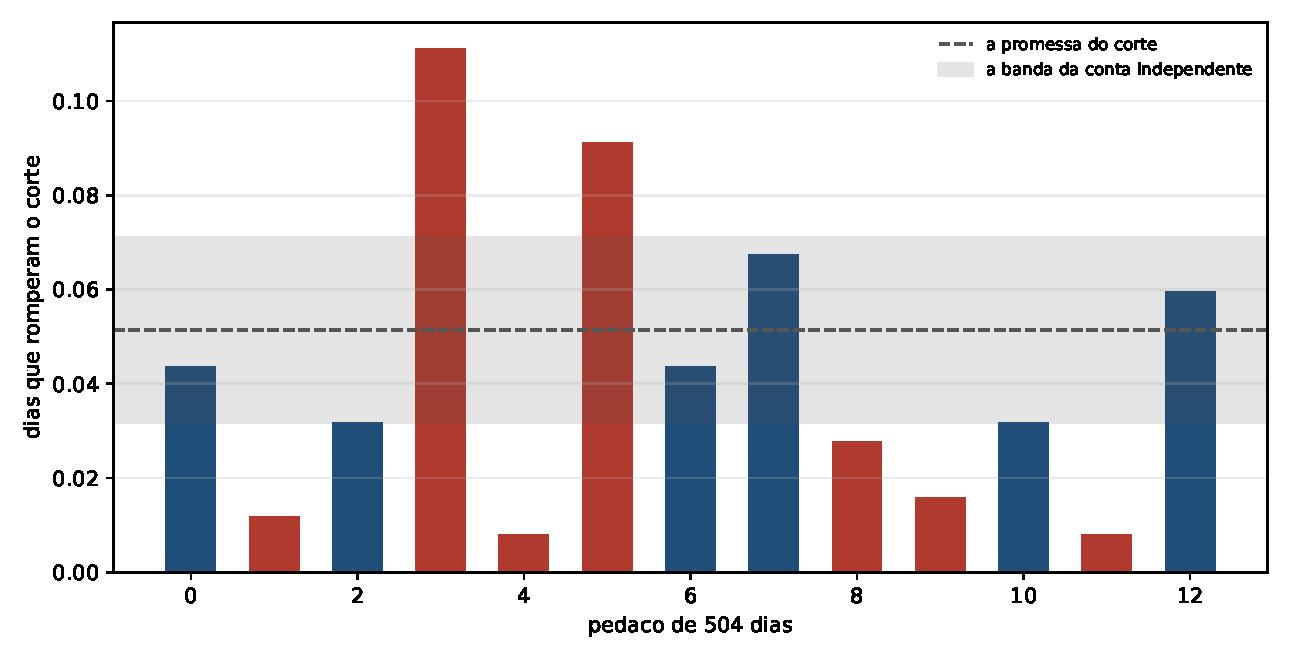
\includegraphics[width=\linewidth]{figuras/E18_o_pedaco_escolhido_1.pdf}
  \caption{A entrega do corte em cada pedaço de \numPedacoMenor{} dias. A linha tracejada é a
    promessa e a faixa cinza é a banda de quem supõe dias independentes. As barras em vermelho são os
    pedaços que caem fora da banda.}
  \label{fig:entrega-por-pedaco}
\end{figure}

Dos \numPedacoPedacosDoisAnos{} pedaços, \numPedacoEntregaForaDoisAnos{} ficam fora da banda de dois
desvios da conta independente, contra \numPedacoEntregaForaCincoAnos{} nos de cinco anos e
\numPedacoEntregaForaDezAnos{} nos de dez --- embora ali só existam \numPedacoPedacosDezAnos{} pedaços,
e duas respostas não façam dispersão. Se os dias fossem independentes, a fração fora seria de cerca de um em
vinte.

\section{Nem tudo balança}

Seria fácil concluir que nada se mede. Não é o que a segunda medição mostra.

A dependência entre as duas pernas --- quantas vezes elas rompem juntas, contra o que a independência
previria --- foi medida nos mesmos pedaços, e ela não se comporta como a entrega do corte.

\begin{table}[htbp]
  \centering
  \small
  \begin{tabular}{rrrr}
    \hline
    pedaço & menor & maior & pedaços sem \\
    (dias) & dependência & dependência & dependência \\
    \hline
    \numPedacoMenor{} & \numPedacoDependenciaMenorDoisAnos & \numPedacoDependenciaMaiorDoisAnos & \numPedacoDependenciaAbaixoDoisAnos \\
    mil duzentos e sessenta & \numPedacoDependenciaMenorCincoAnos & \numPedacoDependenciaMaiorCincoAnos & \numPedacoDependenciaAbaixoCincoAnos \\
    dois mil quinhentos e vinte & \numPedacoDependenciaMenorDezAnos & \numPedacoDependenciaMaiorDezAnos & \numPedacoDependenciaAbaixoDezAnos \\
    \hline
  \end{tabular}
  \caption{O excesso de quedas conjuntas em cada pedaço, contra a independência. A última coluna
    conta os pedaços em que a dependência some.}
  \label{tab:dependencia-por-pedaco}
\end{table}

O número anda dentro de uma faixa larga, e a fronteira fica longe: em nenhum dos pedaços ele chega
perto de um, que seria a independência. A conclusão de que as duas pernas caem juntas sobrevive à troca de pedaço; a
conclusão sobre quanto custa a promessa do corte não sobrevive.

\begin{figure}[htbp]
  \centering
  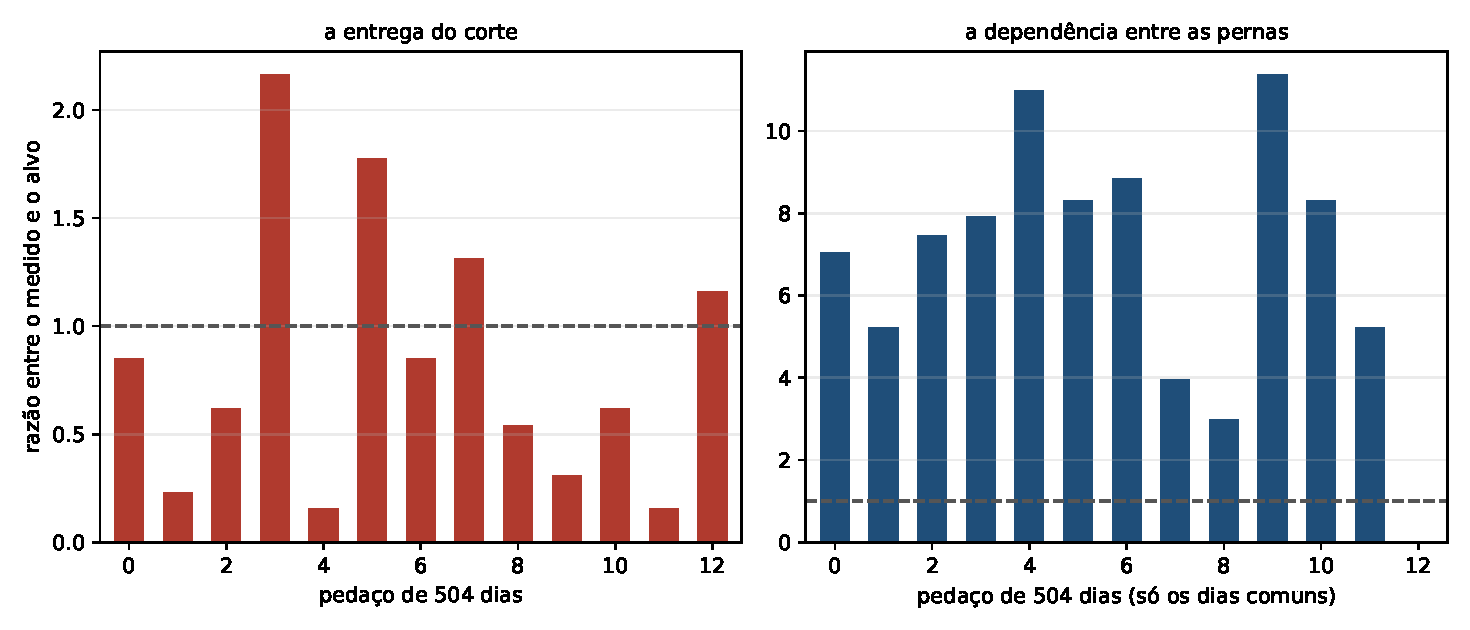
\includegraphics[width=\linewidth]{figuras/E18_o_pedaco_escolhido_2.pdf}
  \caption{As duas conclusões no mesmo tamanho de pedaço, cada uma em razão do seu alvo. À esquerda,
    a entrega do corte, que atravessa a linha da promessa para os dois lados. À direita, a
    dependência, que fica sempre bem acima da independência.}
  \label{fig:duas-conclusoes}
\end{figure}

\section{O que fica}

Fica o primeiro pedaço do enquadramento, e ele é uma regra de relato. Toda resposta sobre uma série
carrega escondida a escolha do pedaço, e a escolha é de quem escreve. O honesto é reportar o par ---
a resposta e a dispersão entre pedaços ---, do mesmo jeito que as medições desta espiral sempre
reportaram a dispersão entre mundos sorteados.

Fica também o que essa disciplina compra, e é mais do que parece: ela \textbf{discrimina}. Com a
dispersão entre pedaços na mão, dá para separar as conclusões que sobrevivem à troca de pedaço das
que não sobrevivem, e as duas aparecem lado a lado na mesma medição. A dependência entre mercados
sobreviveu; o preço da promessa do corte não. Antes desta medição, as duas tinham a mesma cara no
papel.

O andar continua pelo outro corte do enquadramento. A série é cortada no espaço --- onde ela começa e
onde termina --- e é cortada também no \textbf{tempo}: há um instante em que a decisão é tomada, e os
dados com que ela é tomada chegaram antes disso por um tempo que ninguém declarou. Esse é o pedaço
seguinte, e é onde a espiral vai ter de dizer o que é o agora.
